\chapter{Porting Tang}\label{porting-tang}

After successful cross-compilation of José we have all the dependencies packaged except the systemd.
The systemd is only one of many implementations (inetd, launchd, ucspi-tcp, xinetd) of a server providing socket activation.



\section{Socket Activation}\label{socket_activation}

Socket activation is a technology provided by a super-server (also called a service dispatcher daemon).
It uses very few resources when in idle state and starts other services when needed as well, normally with access to them checked by a TCP wrapper.
A service designed for the socket activation would behave as bare CLI application with input read from {\it stdin} (standard input) and output written to {\it stdout} (standard output).
Tang is exactly this kind of application and because of that, we need to configure socket activation.

The xinetd implementation is already packaged for OpenWrt and we will try to configure the Tang to use it later.



\subsection{Xinetd}
xinetd listens for incoming requests over a network and launches the appropriate service for that request.
Requests come to network ports and xinetd usually launches another daemon to handle the request.
This is reflected on Figure \ref{fig_xinetd} xinetd socket activation below.
\begin{figure}[h]
    \centering
    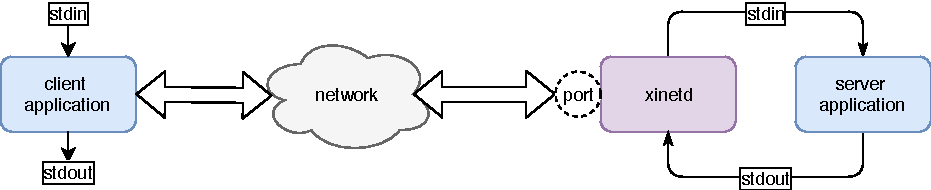
\includegraphics[scale=0.9]{figures/xinetd.pdf}
    \caption{xinetd socket activation}
    \label{fig_xinetd}
\end{figure}
xinetd features access control mechanisms such as TCP Wrapper ACLs (access control lists), extensive logging capabilities, and the ability to make services available based on time.
It can place limits on the number of servers that the system can spawn.
xinetd is listening on behalf of the services.
Whenever a connection comes in, an instance of the respective service will be spawned using {\it stdin} and {\it stdout} of the service application\cite{xinetd}.


\section{Package the Tang}
Similarly to José, we need to create a new package for OpenWrt.
Let us create a branch and {\tt utils/tang} directory where binary programs like Tang belong:
\begin{lstlisting}[columns=fixed,basicstyle=\ttfamily\footnotesize,tabsize=4,backgroundcolor=\color{yellow!10}]
$ git chechout -b add-tang master
$ mkdir -p utils/tang/
\end{lstlisting}
The Tang project is owned by the same owner on GitHub as José.
We should visit the project releases page\footnote{https://github.com/latchset/tang/releases/} and get the Tang version v6.
Then add following lines to the Makefile similarly as with José's Makefile:
\begin{lstlisting}[columns=fixed,basicstyle=\ttfamily\footnotesize,tabsize=4,backgroundcolor=\color{yellow!10}]
include $(TOPDIR)/rules.mk

PKG_NAME:=tang
PKG_VERSION:=6
PKG_RELEASE:=1

PKG_SOURCE:=$(PKG_NAME)-$(PKG_VERSION).tar.bz2
PKG_SOURCE_URL:=\
https://github.com/latchset/$(PKG_NAME)/releases/download/v$(PKG_VERSION)/

PKG_HASH:=1df78b48a52d2ca05656555cfe52bd4427c884f5a54a2c5e37a7b39da9e155e3


PKG_INSTALL:=1
PKG_BUILD_PARALLEL:=1

PKG_FIXUP:=autoreconf

include $(INCLUDE_DIR)/package.mk
\end{lstlisting}
Do not forget to add the package description which should have section dependencies filled.
\begin{itemize}
    \item libhttp-parser -- used for parsing HTTP requests.
    \item José -- the library and tool for the JavaScript Object Signing and Encryption.
    \item xinetd (a run-time dependency)
    \item bash (a run-time dependency)
\end{itemize}
The actual build proccess of the Tang does not require xinetd's libraries but will be configured to use its socket activation available in run-time.
The bash dependency is there for the reason that Tang's {\tt tangd-update} and {\tt tangd-keygen} executables are bash scripts.
These scripts are complex and are using data structures that are not available for OpenWrt's default shell - ash.
Having run-time dependencies listed in the Makefile will ensure that they are installed to the device before the Tang.
\begin{lstlisting}[columns=fixed,basicstyle=\ttfamily\footnotesize,tabsize=4,backgroundcolor=\color{yellow!10}]
define Package/tang
  SECTION:=utils
  TITLE:=tang v$(PKG_VERSION) - daemon for binding data to a third party
  DEPENDS:=+libhttp-parser +xinetd +jose +bash
  URL:=https://github.com/latchset/tang
endef
\end{lstlisting}
The Tang package will be present in utils section of the {\tt openwrt/packages} repository.
Let us add a brief description to our new package using description define:
\begin{lstlisting}[columns=fixed,basicstyle=\ttfamily\footnotesize,tabsize=4,backgroundcolor=\color{yellow!10}]
define Package/tang/description
	Tang is a small daemon for binding data to the presence of a third party
endef
\end{lstlisting}
The buildroot should know where to install the Tang's binaries.
Let us define the install section and use the standard tangd binary location as on Fedora OS:
\begin{lstlisting}[columns=fixed,basicstyle=\ttfamily\footnotesize,tabsize=4,backgroundcolor=\color{yellow!10}]
define Package/tang/install
	$(INSTALL_DIR)	$(1)/usr/libexec
	$(INSTALL_BIN)	\
			$(PKG_INSTALL_DIR)/usr/lib/$(PKG_NAME)d*	$(1)/usr/libexec/
endef
\end{lstlisting}
Do not forget the last line which allows the actual "magic" to happen:
\begin{lstlisting}[columns=fixed,basicstyle=\ttfamily\footnotesize,tabsize=4,backgroundcolor=\color{yellow!10}]
$(eval $(call BuildPackage,$(PKG_NAME)))
\end{lstlisting}
We can now merge these changes to feeds and try to build our freshly created Tang package:
\begin{lstlisting}[columns=fixed,basicstyle=\ttfamily\footnotesize,tabsize=4,backgroundcolor=\color{yellow!10}]
$ git commit -a
$ git push --set-upstream origin add-tang
$ git checkout new_pkgs
$ git merge add-tang
\end{lstlisting}
The new package tang will be available in the {\it Extra packages} section of the menuconfig after updating feeds:
\begin{lstlisting}[columns=fixed,basicstyle=\ttfamily\footnotesize,tabsize=4,backgroundcolor=\color{yellow!10}]
$ ./scripts/feeds update packages
$ ./scripts/feeds install tang
$ make menuconfig
$ make package/tang/{clean,compile}
\end{lstlisting}
After the first try to build the tang package, we will encounter the systemd dependency error:
\begin{lstlisting}[columns=fixed,basicstyle=\ttfamily\footnotesize,tabsize=4,backgroundcolor=\color{yellow!10}]
configure: error: Package requirements (systemd) were not met:

No package 'systemd' found

Consider adjusting the PKG_CONFIG_PATH environment variable if you
installed software in a non-standard prefix.
\end{lstlisting}
We did not define systemd dependency for Makefile, but the cross-compilation of the package will try to configure and compile downloaded sources.
Compiler will try to find the systemd dependency, as it is defined as a dependency in the {\tt configure.ac} file in Tang repository.
We shall remove this builtime dependency.

To do so, we will remove a requirement for systemd from the Tang's configure.ac and Makefile.am file.
These patches are too extensive to be demonstrated.
{\tt Makefile\_am.patch} and {\tt configure\_ac.patch} can be found in submitted pull-request files\footnote{https://github.com/openwrt/packages/pull/5447/files} on GitHub.

To have sources patched before the compilation, we have to crate a directory for them in the package's feeds repository we forked on branch containing commit adding the Tang and copy them to the created directory:
\begin{lstlisting}[columns=fixed,basicstyle=\ttfamily\footnotesize,tabsize=4,backgroundcolor=\color{yellow!10}]
$ cd packages-OpenWrt
$ git checkout add-tang
$ mkdir -p utils/tang/patches
\end{lstlisting}
Patches included in this directory are automatically applied on the sources downloaded from the mirror in the build time.

To have these changes in our feeds in buildroot, commit and push them to the add-tang branch.
After these changes have been pushed and merged with {\it new\_pkgs} branch, a rebuild of the tang package will succeed.
Now we have the Tang package ready to be installed on our device.

We are avoiding troubles by using the libhttp-parser in version 2.8.0.
These problems are described in following subsection \ref{porting_problems}.
The most important part after a successful build would be to configure it correctly.



\subsection{Delivering the Tang Package}\label{porting_problems}

The upstream world is not always ideal.
Soon after this porting effort started, OpenWrt upstream was in a bad shape and almost dead for reasons we described in subsection \ref{LEDE}.
The active part of OpenWrt developers decided to focus on LEDE project and submitting a pull-request to the OpenWrt was painful.
Working with outdated buildroot (or an SDK) was not ideal.
We decided to use the upstream version of buildroot after re-merge.
It solved many issues with outdated dependencies that occured.

\paragraph{Outdated buildroot} caused many issues with dependencies, but as we installed the older version of them, the build could be triggered.
The most time consuming thing was to run a build over and over and collect linker and compiler errors and adding additional flags into Makefile such as:
\begin{lstlisting}[columns=fixed,basicstyle=\ttfamily\footnotesize,tabsize=4,backgroundcolor=\color{yellow!10}]
+CFLAGS += -fhonour-copts
+TARGET_CFLAGS += $(FPIC) -std=gnu99
+TARGET_LDFLAGS += -Wl,-rpath-link=$(1)/usr/lib
\end{lstlisting}
Same flags and running a build over an over were happening with José and with the Tang.
In case of Tang, there was one additional TARGET\_CFLAGS option:
\begin{lstlisting}[columns=fixed,basicstyle=\ttfamily\footnotesize,tabsize=4,backgroundcolor=\color{yellow!10}]
-D_GNU_SOURCE
\end{lstlisting}
Without this option Tang was issuing compilation errors with implicit declaration of the functions:
\begin{lstlisting}[columns=fixed,basicstyle=\ttfamily\footnotesize,tabsize=4,backgroundcolor=\color{yellow!10}]
dprintf()
vdprintf()
\end{lstlisting}
Using uptream buildroot solved these issues for good.

\paragraph{libhttp-parser} dependency has been in its latest version 2.7.1 when the effort started.
Unfortunately, building the Tang package with libhttp-parser updated to version 2.7.1 failed on the dependency and has thrown an error:
\begin{lstlisting}[columns=fixed,basicstyle=\ttfamily\footnotesize,tabsize=4,backgroundcolor=\color{yellow!10}]
checking for http_parser.h... no
configure: error: http-parser required!
\end{lstlisting}
We found out that Fedora's package http-parser contains one patch\footnote{https://github.com/nodejs/http-parser/pull/337} to add the functionality required by the Tang to the http-parser.
Actual checking of the header was in configure.ac file of the Tang package:
\begin{lstlisting}[columns=fixed,basicstyle=\ttfamily\footnotesize,tabsize=4,backgroundcolor=\color{yellow!10}]
AC_CHECK_HEADER([http_parser.h], [],
		[AC_MSG_ERROR([http-parser required!])], [
#include <http_parser.h>
#ifndef HTTP_STATUS_MAP
#error HTTP_STATUS_MAP not defined!
#endif
])
\end{lstlisting}
We first considered applying the very same patch from Fedora package to the http-parser in version 2.7.1 in OpenWrt but in the end, the release 2.8.0 solved the dependency error for a {\it HTTP\_STATUS\_MAP} macro.
On the other hand, it brought an another issue:
\begin{lstlisting}[columns=fixed,basicstyle=\ttfamily\footnotesize,tabsize=4,backgroundcolor=\color{yellow!10}]
Package tang is missing dependencies for the following libraries:
libhttp_parser.so.2.8
\end{lstlisting}
Adding a symbolic link to the libhttp-parser's install sections of the Makefile will suffice.
\begin{lstlisting}[columns=fixed,basicstyle=\ttfamily\footnotesize,tabsize=4,backgroundcolor=\color{yellow!10}]
ln -s libhttp_parser.so.$(PKG_VERSION) libhttp_parser.so.2.8
\end{lstlisting}
